\section{如何阅读 GPU 技术白皮书}

欢迎各位。今天，我们将探索图形处理器白皮书的奇妙世界。白皮书本质上是图形处理器架构的数据表或深入技术规格说明书。这些文档
即白皮书，在比较不同图形处理器时具有无可估量的价值，因为他们提供了对每个架构规格和能力的详细洞察。回到这里的表格，你会注
意到针对每个架构，我们都有一个基于该架构的芯片示例。

\begin{figure}
    \centering
    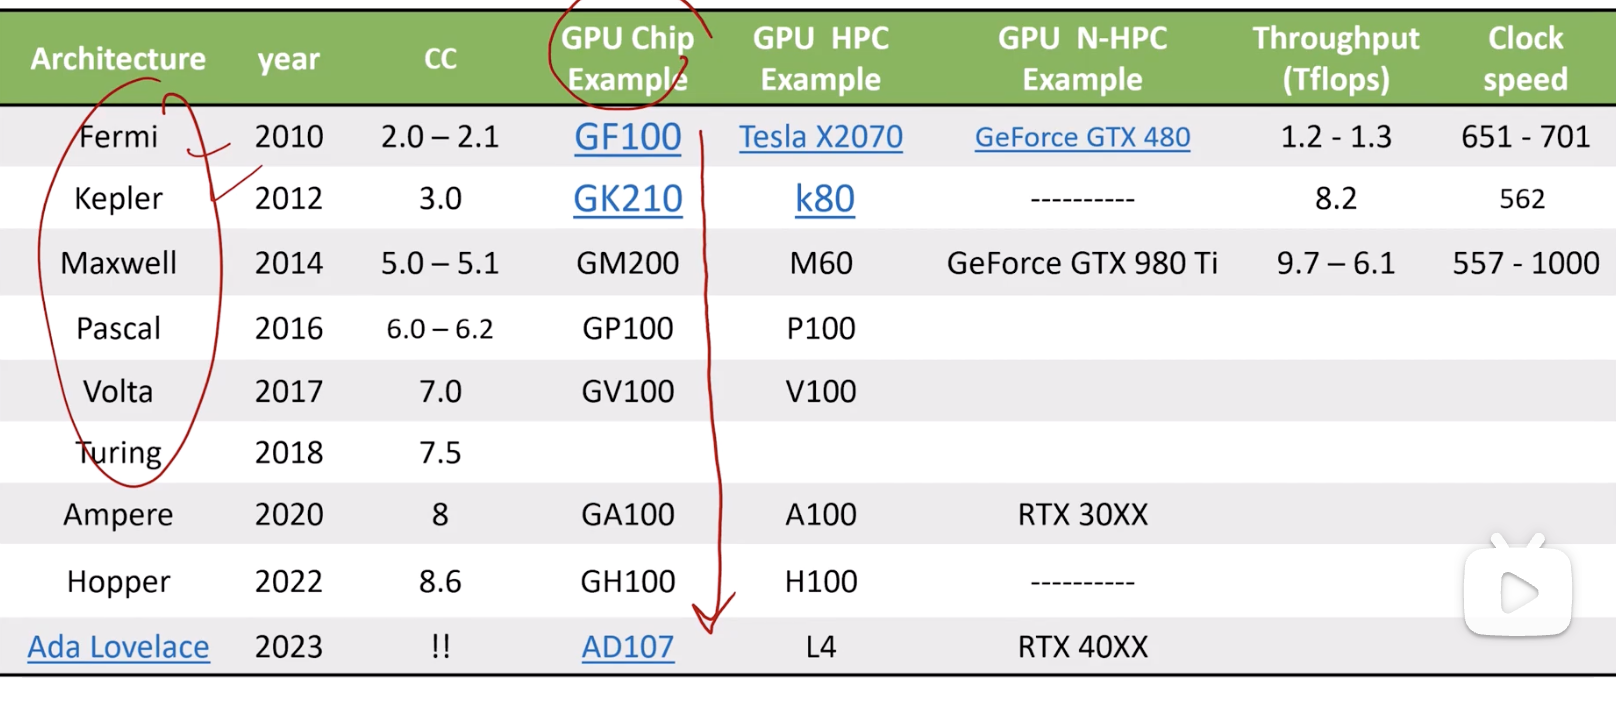
\includegraphics[width=0.75\linewidth]{resources/cuda-044.png}
    \caption{GPU 架构}
    \label{fig:placeholder}
\end{figure}

\subsection{搜索白皮书}

要获取任何架构的白皮书，只需要一次简单的互联网搜索。只需打开你的浏览器，输入芯片名称后加上白皮书一词，而芯片名称可以从这
个表格中过去。这很简单，一旦你这样做了，你很可能就能找到你想要的东西。你可以搜索表格中的芯片名称GF100，然后加上白皮
书。完成这一步后，点击回车，你将看到一系列搜索结果。

\begin{figure}
    \centering
    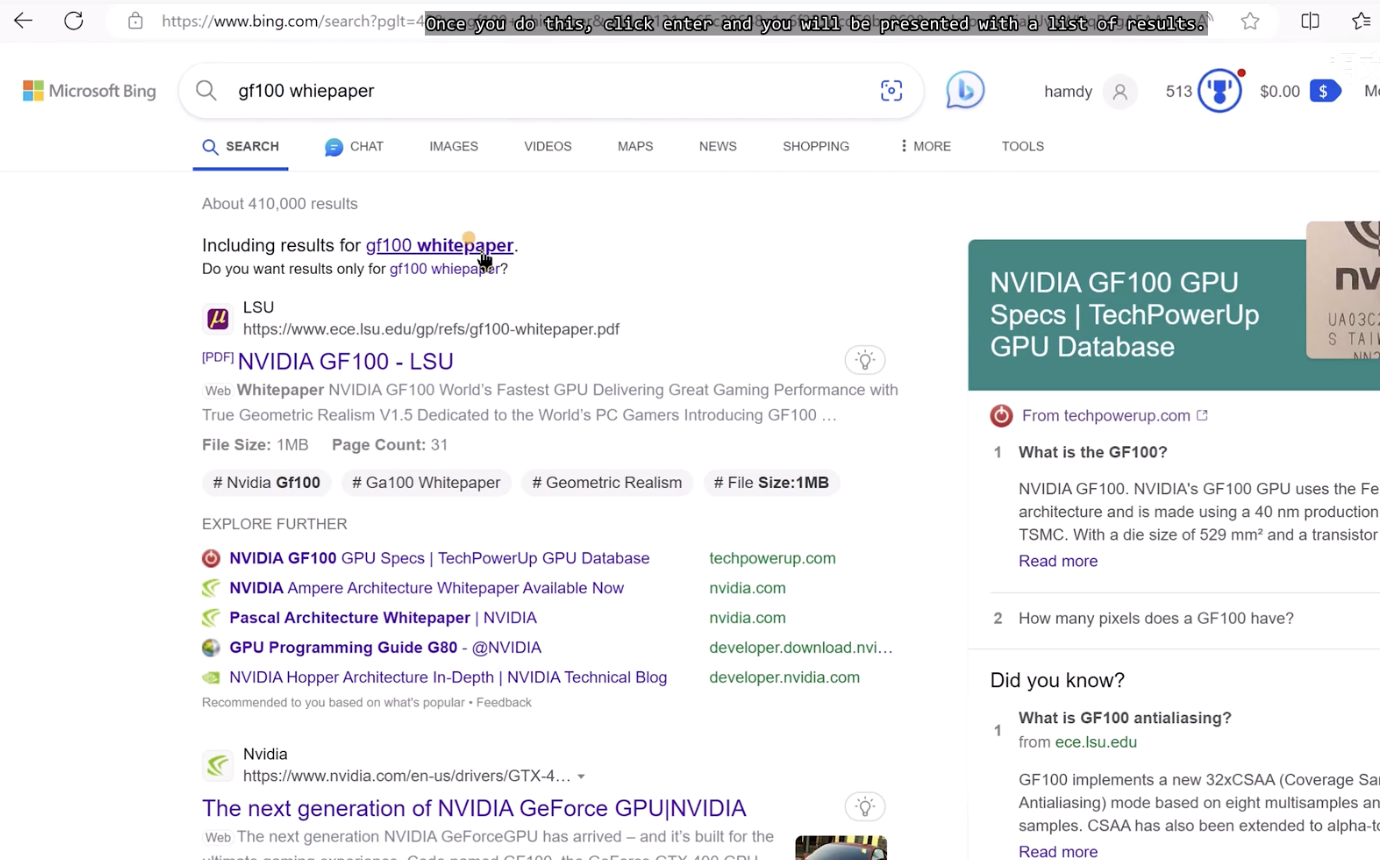
\includegraphics[width=0.75\linewidth]{resources/cuda-045.png}
    \caption{搜索白皮书}
    \label{fig:placeholder}
\end{figure}


你需要寻找那个代表官方白皮书的PDF文件。正如你所见，我们找到了GF100芯片的白皮书。请记住，你寻找的链接应该指向一份
包含完整技术规格的PDF文档。同样地，如果你在研究安培架构，你会搜索GA100白皮书。因为有时你可能会偶然看到文章或总结
，但你真正想要的是原始的全篇白皮书。如你所见，我们拿到了GA100芯片白皮书的PDF文件，让我带你在本文章中了解另一个要
点。英伟达有一个很有帮助的做法，就是在其白皮书中将新架构与旧架构进行比较，以及Pascal架构即V100和P100的性能
比较。如果你正在阅读A100图形处理器或GA100芯片或Ampere 架构的白皮书，你很可能会发现他与前任架构。


\begin{figure}
    \centering
    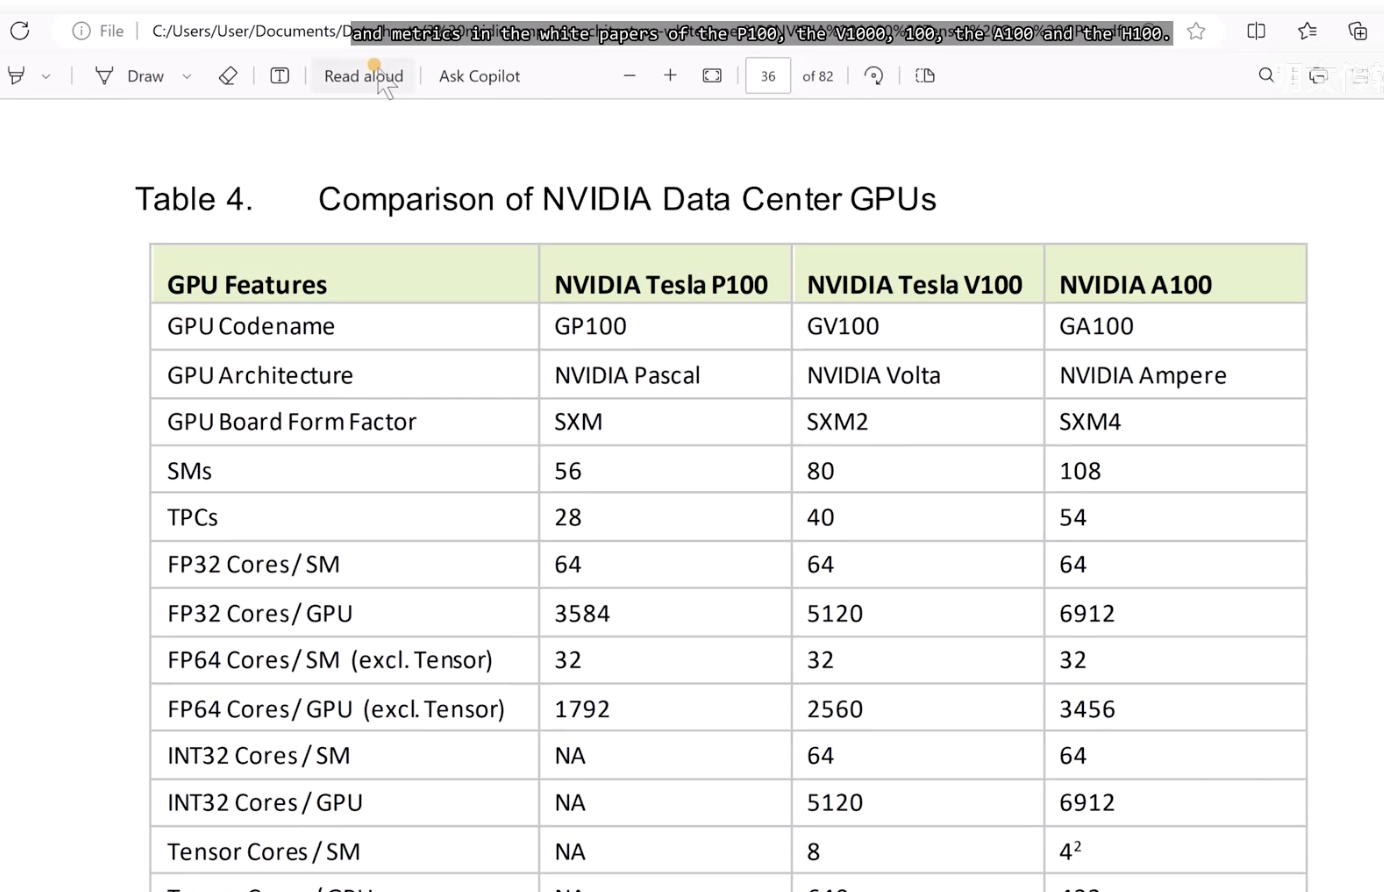
\includegraphics[width=0.75\linewidth]{resources/cuda-046.png}
    \caption{架构比较}
    \label{fig:placeholder}
\end{figure}

例如，你可能会在P100、V100。这就是为什么我们观察到一个有趣的现象，即某些表格和图表可以在不同的白皮书中找到。
A100和H100的白皮书中看到展示不同单元和指标的同一个表格。但我告诉你，正如你现在所见，所有白皮书中的这种一致性意味着一
旦你理解了如何浏览并解读一份英伟达白皮书，那么你就具备了理解其他白皮书的能力。

\subsection{白皮书的结构}

这还不止于此，英伟达的白皮书通常遵循标准化的结构，按顺序包含以下要点，第二点是流式多处理器的内部组件和结构。第一点是新特
性的介绍，第三点是性能基准测试与比较，最后一点是技术规格。让我们从第一点开始，新特性的介绍。每份白皮书都以一个突出展示新
技术和增强功能的部分开始。这可以是任何内容从用于人工智能计算的新型核心，如张量核心，到改进的图形着色技术，甚至是软件或硬
件的任何增强。

\begin{figure}
    \centering
    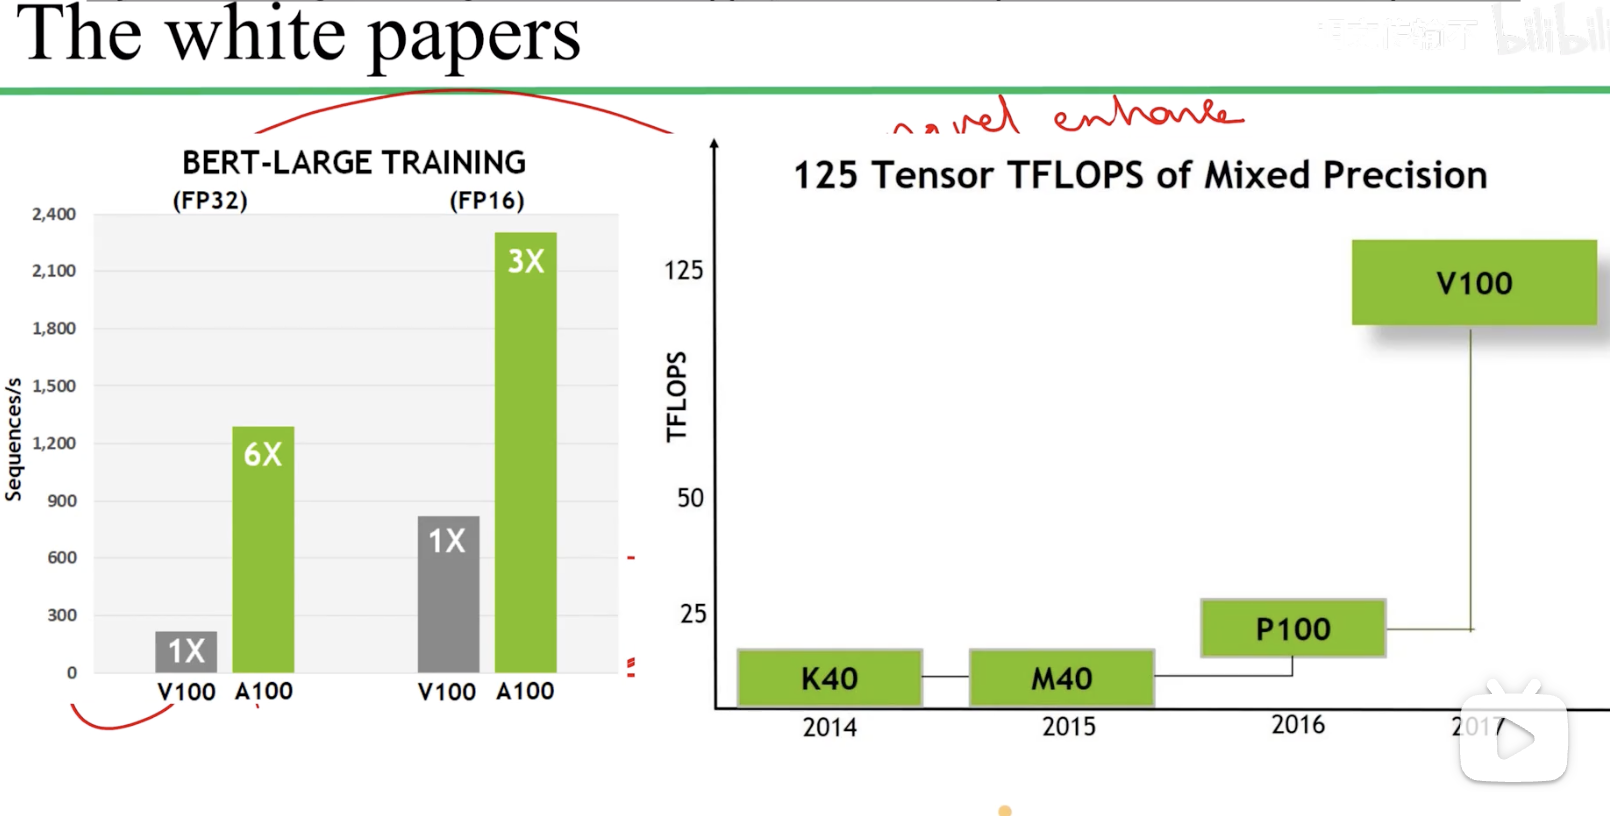
\includegraphics[width=0.75\linewidth]{resources/cuda-047.png}
    \caption{架构比较}
    \label{fig:placeholder}
\end{figure}


第二点是流式多处理器的内部结构或组件。然后是性能基准测试比较。所有白皮书都会深入探讨新型流式多处理器的架构。正如你在我从
不同白皮书中拿来的这些图片中所见，每个架构与其前任都有不同的比较。最后是技术规格，这就是你在每份白皮书中将找到的四个主要
要点。在所有白皮书中都包含详细规格，如核心数量、内存大小、内存带宽、内存技术、功耗要求，以全面展示图形处理器的能力。

\subsection{SM内部结构}

我们将重点关注第二点，计流式多处理器的内部结构。从流式多处理器的内部结构或内部组件开始，英伟达的白皮书深入剖析了每个图形
处理器的流式多处理器设计。接着是我们已经讨论过的通用对比表。例如如果你查看基于Pascal架构的P100图形处理器的白皮
书，即GA100芯片的白皮书，你会注意到这里有一张展示整个图形处理器的图片，然后是流式多处理器的详细图表及其内部组件，如
CUDA核心和内存层级的描述层级。例如我们这里有整个图形处理器，然后有对比表，当我们转向V100白皮书或福特架构白皮书时
会发现类似的布局。最后是流式多处理器的内部结构或内部组件。然而在这里你会观察到一个显著的增强，既增加了张量核心单元。正如
你在这里看到的，Volta架构中有了张量核心单元，但在 Pascal 架构中则没有这样的单元。

让我们继续看A100白皮书或 Ampere架构白皮书。同样这份白皮书展示了整个图形处理器，然后我们看到了流式多处理器内部
结构的详细信息。但我们没有对比表，因为他们把对比表移到了另一个部分。但无论如何，我们在白皮书中还是能看到它。然后正如你所
见，Ampere架构的布局可能看起来有些熟悉，因为它与福特架构中流式多处理器的内部结构非常相似。只要看看这里的这两张图片
，你就会发现没有巨大的变化。

当我们查看H100白皮书或Hopper白皮书时，这种一致性依然存在。然后这个图形处理器架构后面跟着流式多处理器内部结构的
详细信息，这份白皮书呈现了整个图形处理器，正如你在这里看到的，如你所见，这个架构与所有前任架构的主要区别在于每个流式多处
理器中可用的核心数量。例如，你可以数一下在这个架构中有多少个32位浮点核心。并将其与比方说A100图形处理器进行比较，看
看差异。

\begin{figure}
    \centering
    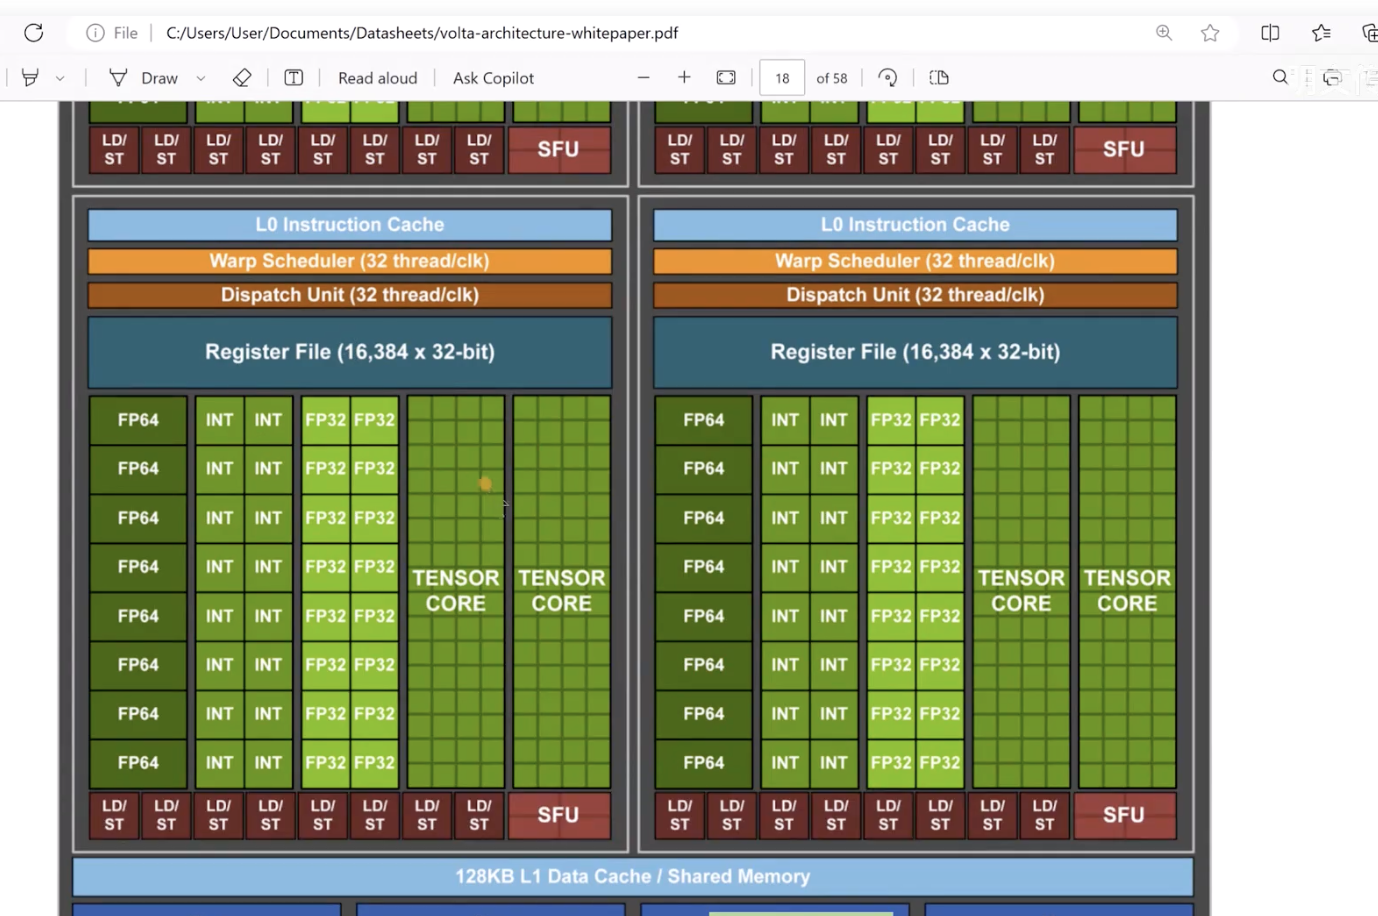
\includegraphics[width=0.75\linewidth]{resources/cuda-048.png}
    \caption{Volta 架构}
    \label{fig:placeholder}
\end{figure}

现在总结一下，我想说的是，虽然每份白皮书都针对其特定的图形处理器，但所有白皮书提供的结构和信息类型都遵循相似的模式。这种
延续性和一致性不仅使专业人员更容易跟上最新技术。而且有助于清晰的理解技术的进步，以及每个新架构与其前任相比的定位。
